\chapter{相关工作}\label{chp:related_work}

本章主要介绍与本文研究内容密切相关的代表性工作与技术基础，为后续章节中方法的提出与分析提供必要的背景支撑。围绕基于内部表征的大语言模型幻觉检测这一主题，本文的研究内容主要涉及通用场景下基于模型内部表征的白盒幻觉检测，以及检索增强生成场景下围绕外部知识利用建模的RAG幻觉检测。本章将从以下三个方面对相关工作进行梳理。

\section{基础概念与技术}\label{sec:llm_rag_sae_background}

本文围绕基于内部表征的大语言模型幻觉检测展开研究，其中第一项工作关注通用场景下大语言模型内部表征中的幻觉信号挖掘，第二项工作则进一步面向检索增强生成场景，研究模型内部知识与外部检索知识之间的冲突及其检测问题。因此，在展开后续方法介绍之前，有必要对大语言模型（Large Language Models, LLMs）、检索增强生成（Retrieval-Augmented Generation, RAG）以及稀疏自编码器（Sparse Autoencoder, SAE）的基本原理进行简要说明，以为后文方法设计提供统一的技术背景。

\subsection{大语言模型基础}

大语言模型通常是指基于大规模语料进行预训练、并具备通用语言理解与生成能力的一类深度神经网络模型\cite{vaswani2017attention,devlin2019bert,radford2018improving}。当前主流的大语言模型大多建立在Transformer\cite{vaswani2017attention}架构之上，能够根据给定上下文预测后续文本内容，并以自回归方式逐步生成完整输出。

对于大语言模型而言，模型输入输出的最基本处理单位称为词元（token）。一个token可以是一个字、一个词、一个词的一部分，或是一个标点符号，其具体形式取决于模型所采用的分词器设计。大语言模型的输入、输出以及内部计算过程，本质上都是围绕token序列展开的。

从结构上看，一个典型的大语言模型通常可以分为输入嵌入层（embedding layer）、若干层堆叠的Transformer模块以及最终输出层三个部分。首先，输入文本在经过分词器切分为离散的token序列后，会被映射为连续向量表示，这一过程由embedding层完成。embedding层的作用是将原本离散的符号编码为模型可以处理的稠密向量，并结合位置信息，使模型能够感知各token在序列中的先后关系。

随后，这些向量表示会进入多层堆叠的Transformer模块中进行逐层加工。每一层Transformer通常包含多头自注意力机制（Multi-Head Self-Attention）和前馈神经网络（Feed-Forward Network）等基本组成部分。自注意力机制负责建模序列中不同token之间的依赖关系，使模型能够根据上下文动态调整对不同位置的关注程度；前馈网络则进一步对每个位置上的表示进行非线性变换和特征提炼。通过这种多层堆叠结构，模型可以逐步将浅层的词法、局部上下文信息，转化为更高层次的句法、语义乃至知识相关表示。公式~\ref{eq:transformer}刻画了单层Transformer模块的基本计算流程。首先，自注意力模块对输入序列中的各位置表示进行上下文交互；随后，通过残差连接与层归一化得到中间表示；再经过前馈网络进行逐位置的非线性特征变换；最后再次通过残差连接与层归一化得到该层输出。这样的结构使模型能够同时建模token之间的依赖关系以及单个位置表示的深层语义变换。
\begin{equation}\label{eq:transformer}
\begin{aligned}
\mathbf{H}^{(l)}_{\mathrm{attn}} &= \mathrm{Attention}\!\left(\mathbf{X}^{(l)}\right), \\
\widetilde{\mathbf{X}}^{(l)} &= \mathrm{LayerNorm}\!\left(\mathbf{X}^{(l)}+\mathbf{H}^{(l)}_{\mathrm{attn}}\right), \\
\mathbf{H}^{(l)}_{\mathrm{mlp}} &= \mathrm{MLP}\!\left(\widetilde{\mathbf{X}}^{(l)}\right), \\
\mathbf{X}^{(l+1)} &= \mathrm{LayerNorm}\!\left(\widetilde{\mathbf{X}}^{(l)}+\mathbf{H}^{(l)}_{\mathrm{mlp}}\right).
\end{aligned}
\end{equation}

在最后一层，模型会将当前隐藏表示送入输出头（通常也称语言建模头、分类头或LM head）进行线性映射，并得到对词表中各候选token的预测分数。经过softmax归一化后，模型即可得到下一个token的概率分布，并据此选择或采样出当前时刻的输出token。重复这一过程，模型便能够逐token生成完整回答。形式化地，设大语言模型记为$M$，则其生成过程可以表示为
\begin{equation}
P_{M}(Y|X)=\prod_{t=1}^{m}P(y_t|X,y_{<t}),
\end{equation}
其中$Y=\{y_1,y_2,\ldots,y_m\}$为模型输出序列，$y_{<t}$表示第$t$个位置之前已经生成的token。该式表明，大语言模型本质上通过条件概率分解实现序列生成，即每一步预测都依赖于输入文本及此前已经生成的上下文。常见的大语言模型架构如图~\ref{fig:llm_architecture}\cite{wolfe2024decoder}所示。

\begin{figure}[htbp]
    \centering
    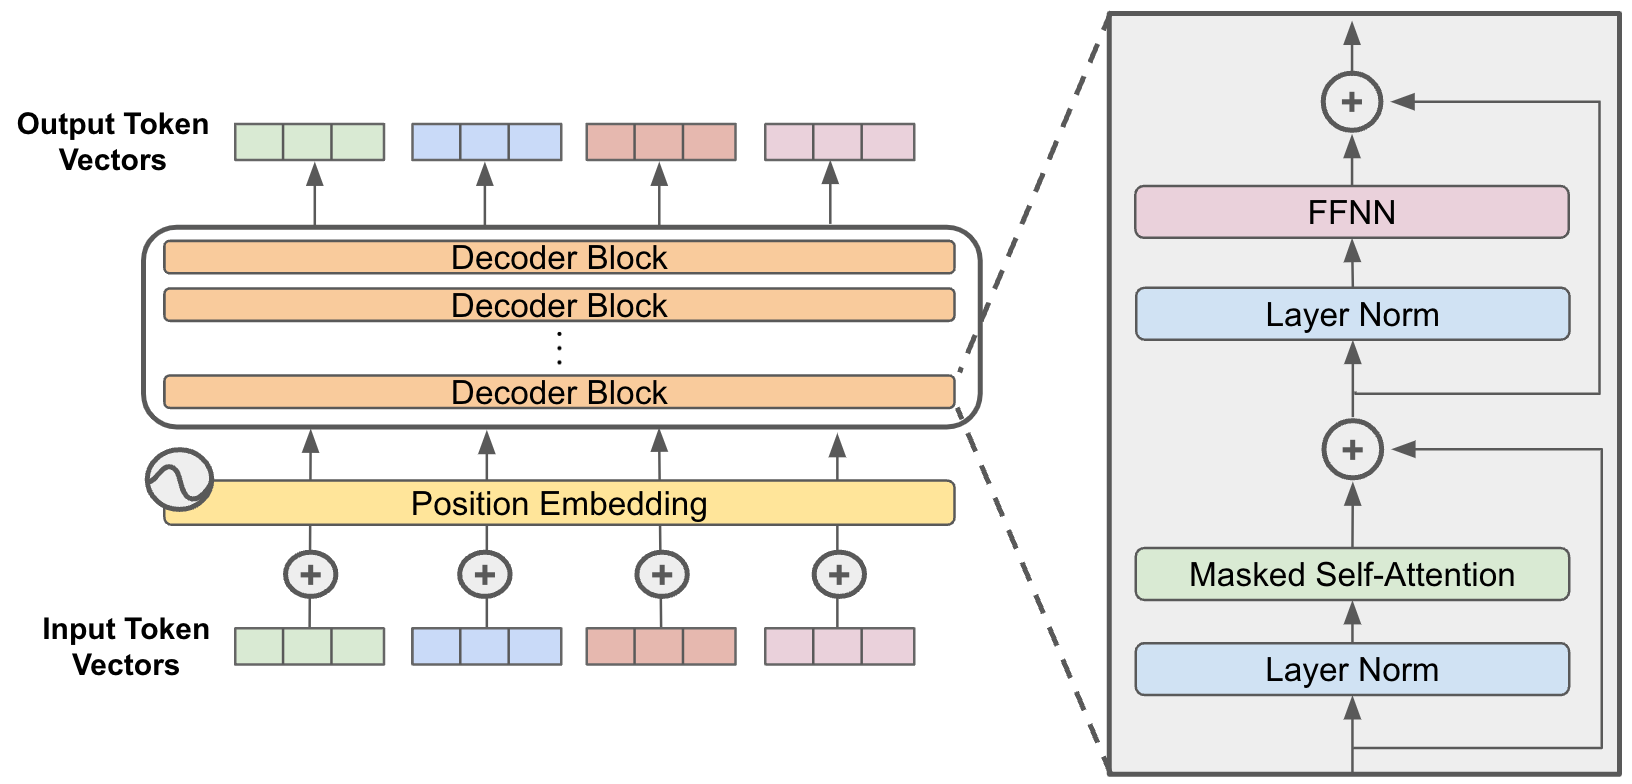
\includegraphics[width=\textwidth]{figures/content/LLM架构.png}
    \caption{大语言模型架构图}\label{fig:llm_architecture}
\end{figure}

需要指出的是，在上述生成过程中，大语言模型不仅会输出最终的文本结果，同时还会在不同层、不同位置产生大量中间表示。广义上说，层间的隐藏状态表示（即$\mathbf{X}^{(l)}$）、Transformer层内部的某些激活值、注意力输出以及前馈网络中的中间激活（如$\mathbf{H}^{(l)}_{\mathrm{attn}}$、$\mathbf{H}^{(l)}_{\mathrm{mlp}}$），都可以视为模型的内部表征（internal representations）。这些内部表征反映了模型对输入语义、上下文约束以及参数化知识的逐步加工过程，是理解模型行为的重要信息来源。当前大多数已有幻觉检测研究工作及本文工作均主要关注并使用各层输出位置上的隐藏向量表示，也可将其理解为经过层间演化后的embedding表征。

\subsection{检索增强生成基本流程}

尽管大语言模型具有较强的参数化知识记忆能力，但其知识更新速度有限，在开放域问答、事实核查、知识密集型生成等任务中，仍可能产生依据不足或与事实不符的内容。为缓解这一问题，研究者提出了检索增强生成框架\cite{gao2024retrieval,huang2024survey,wu2025retrieval}。该框架的核心思想是在模型生成之前，先从外部知识库中检索与当前问题相关的参考材料，再将这些材料与原始问题一同提供给大语言模型，从而使生成过程不再仅依赖模型参数中固有的知识，而是能够显式参考外部证据。

从基本流程上看，RAG通常可概括为“检索—增强—生成”三个阶段。首先，系统根据用户提出的问题，从文档库、网页库、数据库或其他外部知识源中召回若干相关文本片段；其次，将这些检索结果与原始问题按照预设模板进行组织和拼接，构造成增强后的上下文输入；最后，大语言模型基于这一增强后的输入生成最终回答。换言之，RAG并不是直接让模型“凭记忆作答”，而是先“查资料”，再“结合资料作答”\cite{lewis2020retrieval,borgeaud2022improving,lazaridou2022internet}。例如，在医疗问答场景中，用户询问某种疾病的常见治疗方案时，RAG系统可以先检索最新的临床指南、医学百科条目或专业资料，再让模型基于这些检索证据进行归纳生成，从而降低模型直接凭借过时记忆作答的风险。典型的RAG流程如算法~\ref{alg:rag_framework}所示。

\begin{algorithm}[htbp]
\caption{检索增强生成（RAG）基本流程}
\label{alg:rag_framework}
\begin{algorithmic}[1]
\Require 用户输入文本 $X$；外部知识库 $\mathcal{D}$；检索器 $\mathcal{R}$；大语言模型 $M$；返回文档数 $N$
\Ensure 模型生成响应 $Y$

\State 根据用户输入 $X$ 生成检索查询 $q$
\State 利用检索器 $\mathcal{R}$ 在知识库 $\mathcal{D}$ 中召回与 $q$ 最相关的前 $N$ 个文档
\State 得到候选检索结果集合 $R=\{D_1,D_2,\ldots,D_N\}$
\State 对检索结果进行排序、截断或拼接，得到最终参考文档集合 $\widetilde{R}$
\State 将用户输入 $X$ 与参考文档集合 $\widetilde{R}$ 按提示模板组织为增强上下文 $\widetilde{X}$
\State 将增强上下文 $\widetilde{X}$ 输入生成模型 $M$
\State 模型基于增强上下文 $\widetilde{X}$ 逐token生成输出序列 $Y$
\State \Return $Y$

\end{algorithmic}
\end{algorithm}

相较于只依赖参数化知识的生成方式，RAG的优势在于能够引入更实时、更外显、也更可追溯的知识来源，因此在许多知识密集型任务中能够提升回答的事实性和可解释性。然而，RAG并不能从根本上消除幻觉现象。一方面，检索器本身可能召回不完整、不准确或相关性不足的文档；另一方面，即使外部检索结果已经提供了正确信息，生成模型也未必能够始终严格遵循这些证据。特别是在模型内部参数知识与外部检索知识不一致时，模型可能更倾向于依赖自身已有知识，忽略甚至误解检索内容，最终生成与检索证据不一致的回答。

也正因为如此，RAG幻觉检测不再只是单纯判断“模型答得对不对”，而是需要进一步分析“模型是依据什么知识答出来的”“输出与检索证据之间是否一致”“模型内部知识是否压制了外部知识”等更复杂的问题。本文第四章的工作正是在这一背景下展开，试图通过分析模型内部表征与检索内容之间的关系，更直接地刻画RAG场景中的知识冲突现象，并据此进行幻觉检测。

\subsection{稀疏自编码器基础}

为了进一步挖掘大语言模型内部隐藏状态中的可解释判别信息，近年来研究者开始关注利用稀疏表示学习方法对原始隐藏状态进行重构与解耦。其中，稀疏自编码器（Sparse Autoencoder, SAE）\cite{shu2025survey,ng2011sparse,bricken2023towards,huben2024sparse}是一类具有代表性的表征学习模型，其目标是在尽可能保留输入信息的同时，将原始稠密表示映射到更高维、但更加稀疏的特征空间中。

一般而言，自编码器由编码器和解码器两部分组成。给定输入向量$\mathbf{h}\in\mathbb{R}^{d}$，编码器首先将其映射为潜在特征$\mathbf{z}\in\mathbb{R}^{D}$，$\mathbf{z}=f_{\mathrm{enc}}(\mathbf{h})$，其中通常有$D>d$。随后，解码器再根据$\mathbf{z}$重构输入$\hat{\mathbf{h}}=f_{\mathrm{dec}}(\mathbf{z})$。模型训练的目标是在减小重构误差的同时，对潜在表示$\mathbf{z}$施加稀疏约束，使得每个样本仅激活少量特征维度。对应的优化目标一般可写为
\begin{equation}
\mathcal{L}=\|\mathbf{h}-\hat{\mathbf{h}}\|_2^2+\lambda \,\Omega(\mathbf{z}),
\end{equation}
其中第一项为重构损失，第二项为稀疏正则项，$\lambda$用于平衡二者，$\Omega(\mathbf{z})$可取$L_1$范数等形式，令$\mathbf{z}$在大多数维度上为0。

相较于原始隐藏状态，SAE得到的稀疏特征通常具有两方面优势。其一，原始隐藏状态中的语义信息往往高度纠缠，不同维度混合承载多种语义因素，而稀疏映射有助于将这些纠缠信息分解为相对独立的特征单元，从而增强表示的可解释性。其二，稀疏特征在后续统计筛选和下游建模中通常更易处理。例如，可以在高维稀疏特征空间中计算各特征维度与标签之间的关联程度，筛选出最具判别力的特征子集，并进一步利用简单、可解释的分类模型进行建模。

~\newline

以上内容从整体上介绍了本文后续研究所主要依赖的三项基础技术。大语言模型为幻觉检测提供了研究对象及其内部表征来源；RAG框架通过引入外部检索知识扩展了生成条件，也使幻觉检测从单纯的输出正确性判断进一步发展为对内外知识关系的建模；SAE则为从复杂隐藏状态中提取高维、稀疏、可解释的判别特征提供了有效工具。三者共同构成了本文两项方法研究的技术基础：前者支撑ATScore对内部表征动态结构的建模，后两者则共同支撑SKID对RAG场景下知识冲突信号的提取与解释。

\section{基于内部表征的幻觉检测}\label{sec:white_box_hallucination_detection}

% 方法一基于CoE缝合ACT-ViT，所以要介绍这两个。
% 介绍INSIDE、ITI、SAPLMA、CoE、ACT-ViT方法。分为两类：需要训练vs不需训练。
% INSIDE、CoE属于不用训练的方法，ITI、SAPLMA、ACT-ViT属于需要训练的方法。

大语言模型幻觉通常指模型生成的内容虽然在语言形式上流畅自然，但在事实层面与真实世界知识、给定上下文或问题语义不一致的现象。围绕这一问题，幻觉检测任务旨在根据模型生成过程中的相关信号，对当前输出是否包含幻觉进行判断。根据可利用信息来源的不同，现有方法大致可分为黑盒方法与白盒方法两类。前者通常仅依赖输入文本、生成结果或外部辅助信息进行判别；后者则进一步利用模型推理与生成过程中的内部状态信息，如隐藏状态、激活值、logits及中间层表征等，从模型内部挖掘能够反映生成真实性的判别信号。

从基本思路上看，白盒幻觉检测通常可概括为如下过程：首先，在模型生成阶段提取特定层、特定位置或特定类型的内部表征；随后，基于这些表征构造能够反映生成可靠性的特征或判别分数；最后，根据这些特征或分数对输出进行幻觉检测。按照是否需要额外训练检测模块，现有白盒方法又可进一步分为两类：一类方法不依赖额外训练，而是直接从内部状态中构造统计量、一致性指标或启发式分数；另一类方法则利用带标注数据对内部表征进行探测、分类或干预，以学习更具判别性的幻觉检测模型。

尽管白盒方法为幻觉检测提供了比黑盒方法更丰富的可用信息，但其仍面临若干关键挑战。一方面，大语言模型的内部状态维度高、层数深，包含大量冗余甚至噪声信息，如何从中定位真正与幻觉相关的判别特征并非易事；另一方面，不同层、不同token位置以及不同表示形式所蕴含的信息存在显著差异，如何设计有效的特征提取与利用方式，仍是当前白盒幻觉检测研究中的核心问题。基于此，现有工作围绕内部表征的利用方式提出了多种方案，以下将对其中具有代表性的白盒幻觉检测方法进行分类介绍与分析。

\subsection{无需额外训练的方法}\label{subsec:white_box_no_training}

在白盒幻觉检测研究中，一类具有代表性的方法是不额外引入专门的检测器训练过程，而是直接基于大语言模型生成过程中的内部状态构造启发式判别依据。与依赖监督信号学习分类边界的方法不同，这类方法通常通过分析隐藏状态、跨层表征或生成过程中的一致性特征，直接计算用于表征输出可靠性的分数或指标。其主要优势在于实现简单、部署成本较低，并且避免了额外标注数据和训练过程所带来的模型适配问题，因此在跨模型、跨任务和跨数据集场景下通常具有更好的迁移潜力。

\begin{figure}[htbp]
    \centering
    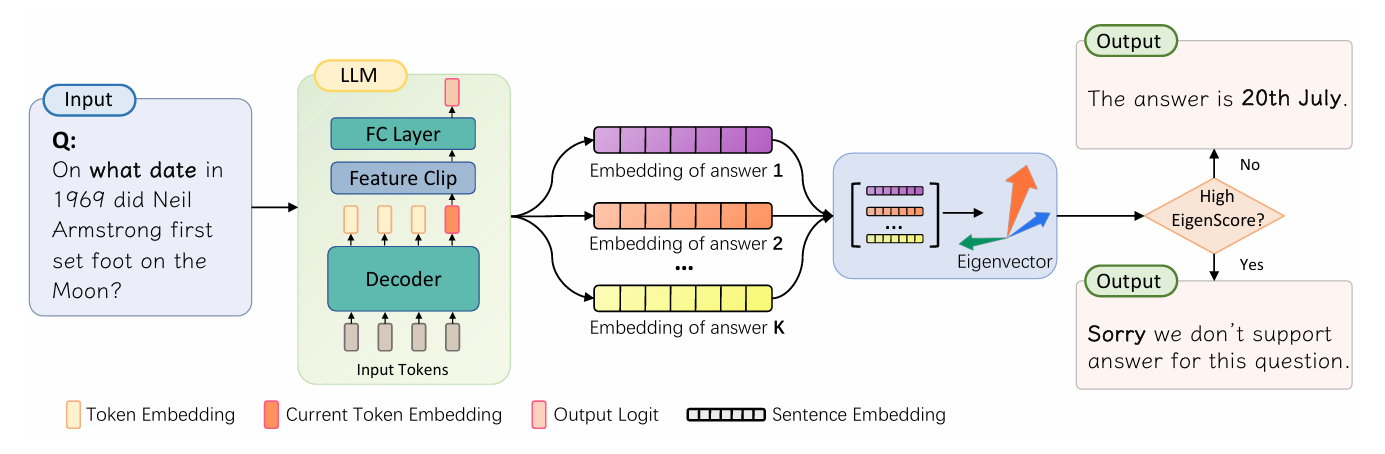
\includegraphics[width=\textwidth]{figures/content/INSIDE框架图.png}
    \caption{INSIDE方法框架图}\label{fig:inside}
\end{figure}

INSIDE\cite{chen2024inside}是一种典型的不依赖额外训练的白盒幻觉检测框架，其方法框架图如图~\ref{fig:inside}所示。该方法的基本出发点在于：当模型对某一问题具有较为稳定和可靠的知识时，多次采样的生成结果在其语义空间中的嵌入表示通常表现出更强的一致性；相反，当模型可能生成幻觉内容时，其内部状态往往会呈现更大的波动性。因此，INSIDE通过考察多次生成条件下中间层表示的一致程度，来衡量模型输出的可靠性，并据此实现幻觉检测。具体地，该方法提出表征幻觉水平的EigenScore指标，其计算过程大致如下：

令大模型对同一问题生成$K$次回答，取每次回答的最后一个token在第$l$层的隐藏状态$h^{l}_k\in\mathbb{R}^{d}$作为整个句子的表征，构成一个表征矩阵$\mathbf{Z}^l=\left [h^{l}_1,h^{l}_2,\ldots,h^{l}_K\right ]\in\mathbb{R}^{d\times K}$。随后，计算协方差矩阵$\bm{\Sigma}^l=\mathbf{Z}^{l\top}\mathbf{Z}^l\in\mathbb{R}^{K\times K}$。对此协方差矩阵作对数行列式计算，即得文章所定义的EigenScore：
\begin{equation}
    \text{EigenScore}=\frac{1}{K}\log \det \left (\bm{\Sigma}^l\right )=\frac{1}{K}\sum_{i}^{K}\log(\lambda_i).
\end{equation}
其中$\lambda$为协方差矩阵$\bm{\Sigma}^l$的$K$个特征值。该指标反映了多次生成结果在内部表征空间中的分布情况，协方差矩阵特征值/对数行列式越大表示生成结果在该层的表征空间中分布越分散，可能对应更高的幻觉风险；反之，较小的特征值则表明生成结果在该层的表征空间中更为集中，可能对应更低的幻觉风险。在实际实验中，层数$l$通常取模型中间层，即总层数之一半$l=L/2$。

CoE\cite{wang2025latent}则代表了另一类无需训练的白盒思路，即直接从模型内部表征中构造可解释的几何或统计特征，并以此作为幻觉检测依据。相较于仅关注单一层、单一token的方法，这类工作更强调从内部表征整体结构中提取能够反映生成真实性的判别线索，且无需对同一问题采样多条输出，显著降低了检测成本。按照本文研究设定，CoE属于无需训练的方法，其核心价值在于不依赖额外标注训练，而是通过对内部表征结构属性的直接刻画实现幻觉判断。该方法大致计算思路如下：

首先定义“embedding链”为各层的embedding表征所组成的序列，即：
\begin{equation}
    \mathbf{H}=h_0\rightarrow h_1\rightarrow\cdots\rightarrow h_L.
\end{equation}
其中，$h_l=\frac{1}{T}\sum_{t=1}^{T}h_l^t\in\mathbb{R}^{d}$为第$l$层的隐藏状态，$d$为隐藏维度，由各输出token平均而来。随后，CoE通过分析embedding链中不同层的表征分布特征，构造了一组基于链式内部表征结构的幻觉检测指标：
\begin{gather}
\text{CoE-R}=\frac{1}{L}\sum_{l=0}^{L-1}\left (\frac{M(h_l,h_{l+1})}{M(h_0,h_L)}-\frac{A(h_l, h_{l+1})}{A(h_0, h_L)}\right ) \\
\text{CoE-C}=\frac{1}{L} \sqrt{\left(\sum_{l=0}^{L-1} M(h_{l}, h_{l+1}) \cos (A(h_{l}, h_{l+1}))\right)^{2}+\left(\sum_{l=0}^{L-1} M(h_{l}, h_{l+1}) \sin (A(h_{l}, h_{l+1}))\right)^{2}}
\end{gather}
其中，$M(\cdot)$和$A(\cdot)$分别为两层表征之间的欧氏距离和由余弦相似度及反三角函数定义的角度。CoE-R指标反映了embedding链中相邻层之间的平均距离和角度之差；CoE-C指标则通过将相邻层之间的距离与角度结合起来，构建了一个综合反映embedding链整体结构特征的指标。当embedding链整体越平整，CoE指标越高，幻觉风险越高；链越卷曲，CoE指标越低，幻觉风险也较低。通过分析这些指标在不同生成结果上的分布情况，CoE能够在无需训练的前提下实现对幻觉输出的有效识别。

~\newline

总体而言，无需训练的白盒幻觉检测方法验证了这样一个重要事实：大语言模型内部表征中确实蕴含着与幻觉高度相关的判别信息，即使不借助额外监督训练，也能够在一定程度上实现有效检测。INSIDE通过表示一致性揭示了内部状态与幻觉之间的关联，CoE则进一步体现了从内部表征结构属性中直接构造检测信号的可行性。与此同时，现有无需训练方法大多仍停留在较粗粒度的计算或启发式建模层面，对于内部表征中更细致、更关键的判别特征挖掘仍显不足，这也为后续研究提供了改进空间。

\subsection{需要额外训练的方法}\label{subsec:white_box_need_training}

与无需训练的方法不同，另一类白盒幻觉检测方法通常利用带标注数据对模型内部表征进行进一步建模，通过训练额外的探测器、分类器或干预模块，从隐藏状态中学习更具判别性的幻觉相关信号。该类方法的基本假设是：大语言模型内部不仅隐含了与生成内容真实性相关的潜在信息，而且这些信息可以通过适当的监督学习过程被更有效地提取出来。相较于直接构造启发式统计量的方法，基于训练的白盒方法通常能够学习更复杂的判别边界，从而在特定任务或数据集上取得更好的检测性能；但与此同时，这类方法也往往需要额外的标注样本、训练开销以及更强的模型适配过程，其泛化能力和可迁移性也可能受到训练分布的影响。

SAPLMA\cite{azaria2023internal}是典型的属于需要训练的白盒方法。与直接利用手工构造统计量不同，该类方法更强调通过监督学习的方式，从隐藏状态中训练专门的判别模块，以识别模型输出是否存在幻觉。其核心思路在于，将生成过程中提取到的内部表示视为与真实性判断相关的特征输入，再借助分类器学习幻觉与非幻觉之间的区分边界。具体地，SAPLMA方法使用一个简单的三层前馈神经网络和ReLU激活函数作为判别器，使用训练数据在大模型特定层上的隐藏表征作为输入，预测其相应的幻觉/非幻觉标签。相比无需训练的方法，SAPLMA能够利用训练数据中的标签信息，从而捕捉更具任务针对性的表征模式。因此，这类方法通常在特定数据集上能够获得较好的检测效果。

ITI（Inference-Time Intervention）\cite{li2023inference}是该类方法中的代表性工作之一。该方法的核心思想在于：大语言模型的内部表征空间中往往存在与“真实性”或“事实性”相关的方向，若能够利用少量标注样本识别出这些方向，便可以在推理阶段对模型内部状态进行干预，从而影响最终输出的真实性表现。从白盒幻觉检测的视角看，ITI表明模型隐藏状态中并非仅包含分布式、难以解释的语义信息，还可能蕴含可被线性探针捕捉的真实性判别结构。

该方法基于一个简单的“探测器”模型：
\begin{equation}
    \label{eq:probe}
    p_\theta(x_l^h)=\text{sigmoid}(\langle\theta,x_l^h\rangle),
\end{equation}
其中$x_l^h$为第$l$层第$h$个注意力头的激活值，$\langle\cdot,\cdot\rangle$表示余弦相似度，$\theta\in\mathbb{R}^d$是可训练参数。在训练集$\{(x_l^h,y)_i\}_{i=1}^N$上，该方法对大模型每一层的每一注意力头均训练一个式~\ref{eq:probe}所示的探测器，训练目标是最大化预测概率$p_\theta(x_l^h)$（表示当前输出是否包含幻觉）与真实标签$y$的交叉熵。训练完成后，得到的参数$\theta$可视为是在该注意力头位置上指向“生成幻觉内容”的方向。既可根据在验证集上的性能选择有最佳判别力的层和注意力头位置，又可根据训练得到的$\theta$参数，在推理阶段对模型内部状态进行干预，引导模型生成更可靠的输出。该方法的重要意义在于，它从更加细粒度（注意力头激活值）的层面探索了幻觉内容的表征信号。

ACT-ViT\cite{bar2025beyond}进一步体现了通过训练机制深度挖掘内部激活信息的思路。该方法不再满足于利用单一层、单一位置或简单统计量来刻画模型状态，而是尝试将更完整的内部激活张量组织为适于学习的表示形式，并借助视觉Transformer模型建模其中的空间关联与判别模式。该方法的框架图如图~\ref{fig:act_vit}所示。

\begin{figure}[htbp]
    \centering
    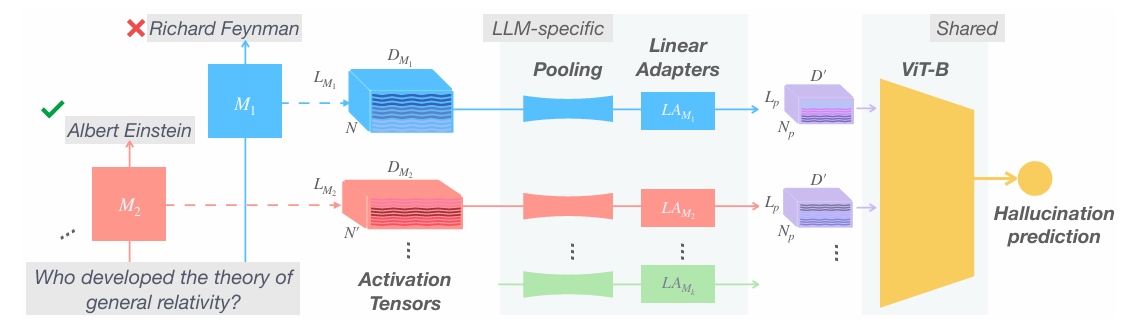
\includegraphics[width=\textwidth]{figures/content/ACT-ViT框架图.png}
    \caption{ACT-ViT方法框架图}\label{fig:act_vit}
\end{figure}

具体地，该方法将大模型在一次前向传播过程中提取到的内部激活张量视作一个具有丰富结构信息的对象：$\mathbf{A}\in\mathbb{R}^{L\times T\times d}$。该张量具有三个维度，其中$L$为大模型层数，$T$为token数量，$d$为大模型内部隐藏维度。该张量涵盖了大模型各层、各位置的内部表征，可以视为是对生成过程的一个全局性建模。作者观察到，此三维张量相较于图像数据，具有类似于图像宽$\times$高$\times$通道的空间结构，因此借鉴视觉Transformer（ViT）的设计思路，构建了一个基于ViT的轻量化判别模型来学习从内部激活到幻觉标签的映射关系。从方法设计上看，ACT-ViT将内部激活视作具有丰富结构信息的对象，强调不同层、不同token位置之间的联合模式对于幻觉检测的重要性。这种思路相较于传统的探针式方法，充分挖掘了大模型所有的内部表征，有助于挖掘隐藏空间中更复杂的幻觉相关模式。与此同时，该方法也指出，既有白盒幻觉检测研究往往仅利用孤立的层或token位置，未能充分挖掘完整内部激活张量中所蕴含的丰富信息。

~\newline

总体来看，需要训练的白盒幻觉检测方法相较于无需训练的方法，通常具备更强的特征学习能力，能够借助监督信号从高维内部表征中提取更具判别性的幻觉相关模式。SAPLMA体现了基于监督分类器直接建模隐藏状态的可能性，ITI验证了在注意力头表征空间中存在可供利用的真实性方向，而ACT-ViT则进一步说明，对完整内部激活结构进行联合建模有助于提升检测性能。然而，这类方法也普遍面临若干共同问题：其一，训练过程需要额外标注数据与计算开销；其二，基于训练的模型可能面临过拟合和泛化性能降低的风险。因此，围绕内部表征的有效表示、特征筛选与判别建模，仍是白盒幻觉检测领域的重要研究方向。

\section{RAG幻觉检测}\label{sec:rag_hallucination_detection}

% 方法二基于RAGLens基础修改。
% 介绍ReDeEP、LUMINA、RAGLens方法。重点关注它们如何利用retrieved context。

检索增强生成（Retrieval-Augmented Generation, RAG）通过在生成前引入外部检索知识，为大语言模型提供与当前问题相关的补充信息，从而缓解仅依赖参数知识时可能出现的事实性错误。然而，外部知识的引入并不意味着幻觉问题被彻底消除。在实际应用中，即使给定了与问题相关的检索上下文，模型仍可能生成与检索内容不一致、未被证据支持，甚至与外部知识相悖的回答。针对这一现象，RAG幻觉检测旨在结合问题、检索文档与生成结果，判断当前输出是否真正得到了外部证据支持。与非RAG场景下的幻觉检测相比，RAG幻觉检测的关键难点在于如何有效利用检索到的外部知识。一方面，检索文档通常包含冗余、噪声甚至相互冲突的信息，模型未必能够准确聚焦于与当前回答最相关的证据；另一方面，生成结果与检索内容之间的关系往往不是简单的词面重合，而涉及更复杂的语义对齐与证据支持关系。因此，如何刻画模型输出与外部知识之间的一致性，消解模型内外知识冲突，并据此识别RAG场景下的幻觉，是当前该方向研究的核心问题。

围绕这一目标，现有研究主要从证据一致性建模、证据支持强度分析以及检索知识利用过程刻画等角度展开探索。ReDeEP\cite{sun2025redeep}是较早关注RAG场景下外部知识利用与参数知识竞争关系的代表性工作之一。ReDeEP认为幻觉的产生往往与两类因素有关：一是模型未能有效保留和利用检索得到的外部知识，二是模型在生成过程中对参数知识产生了过强依赖。为此，该方法分别定义了外部上下文分数（External Context Score, ECS）和参数知识分数（Parametric Knowledge Score, PKS），并将二者结合起来用于幻觉检测。

具体而言，ReDeEP首先利用注意力头对检索文档的关注情况构造外部上下文分数。对于生成的最后一个token，设某一层第$h$个注意力头选出的高注意力上下文token集合为$I_n^{l,h}$，则其token级ECS定义为
\begin{equation}
E_n^{l,h}=\frac{e\cdot x_n^L}{\|e\|\,\|x_n^L\|},\quad
e=\frac{1}{|I_n^{l,h}|}\sum_{j\in I_n^{l,h}}x_j^L,
\end{equation}
其中，$x_n^L$表示最后一层中当前生成token的隐藏状态，$e$表示被该注意力头重点关注的上下文token在最后一层隐藏状态上的平均表示。该分数本质上刻画了当前生成内容与其所关注外部证据之间的语义一致程度：分数越高，说明模型越可能有效利用了检索知识。

在此基础上，ReDeEP进一步将参数知识分数与外部上下文分数进行线性组合，构造最终的幻觉检测分数。其token级检测函数写为
\begin{equation}
H_t(t)=\sum_{l\in F}\alpha P_t^l-\sum_{l,h\in A}\beta E_t^{l,h},
\end{equation}
其中，$P_t^l$表示第$l$层FFN引入的参数知识分数（PKS），$E_t^{l,h}$表示对应注意力头的外部上下文分数（ECS），$F$和$A$分别表示与参数知识和外部知识利用最相关的FFN层与注意力头集合，$\alpha,\beta>0$为回归系数。由此可见，当模型对参数知识的依赖增强而对外部证据的利用减弱时，检测分数会增大，从而更倾向于判定为幻觉。ReDeEP的意义在于，它不再仅从输出文本与检索文档的表层匹配关系出发，而是试图从模型内部机制层面直接地区分“外部知识利用不足”和“参数知识过度介入”这两种因素，从而为RAG幻觉检测提供了更具解释性的分析视角。

LUMINA\cite{yeh2025lumina}同样从“外部上下文利用”与“内部知识利用”两个互补视角对RAG幻觉进行建模。LUMINA分别定义外部上下文利用信号$E_{p_\theta}$与内部知识利用信号$I_{p_\theta}$，并将二者组合为token级幻觉分数：
\begin{equation}
H_t(a_t \mid q,d,a_{<t})
=
\lambda \, I_{p_\theta}(a_t \mid q,d,a_{<t})
-
(1-\lambda)\, E_{p_\theta}(a_t \mid q,d,a_{<t}),
\end{equation}
其中，$q$表示输入问题，$d$表示检索文档，$a_{<t}$表示当前token之前已生成的前缀，$\lambda$为平衡内部知识与外部证据贡献的系数。由此可见，当内部知识利用更强而外部上下文利用更弱时，模型更倾向于被判定为产生幻觉。句子级幻觉分数则可由各token分数进一步求平均得到。

在外部上下文利用的刻画上，LUMINA不再像ReDeEP那样依赖特定注意力头，而是直接比较模型在“相关检索文档”和“随机文档”条件下的下一token预测分布差异。设$P(E_v)=p_\theta(v\mid q,d,a_{<t})$，$Q(E_v)=p_\theta(v\mid q,d',a_{<t})$，其中$d'$表示与问题无关的随机文档，$E_v$表示词表中token $v$对应的嵌入表示，则LUMINA采用最大均值差异（Maximum Mean Discrepancy, MMD）来定义外部上下文利用分数：
\begin{equation}
\begin{aligned}
    E_{p_\theta}(a_t \mid q,d,a_{<t})
    &:=
    \mathrm{MMD}_k^2(P,Q) \\
    &=
    \mathbb{E}_{A,A'\sim P}[k(A,A')]
    +
    \mathbb{E}_{B,B'\sim Q}[k(B,B')]
    -
    2\mathbb{E}_{A\sim P,B\sim Q}[k(A,B)],
\end{aligned}
\end{equation}
其中$k(\cdot,\cdot)$为核函数，文中默认采用余弦核。该式反映了模型预测分布对文档语义变化的敏感程度：若将相关文档替换为随机文档后词表预测分布发生明显变化，则说明模型在生成当前token时更充分地利用了外部检索知识。与此同时，LUMINA还通过跨层信息处理速率来定义内部知识利用信号，以刻画模型在生成过程中对内部参数知识的调用强度。整体而言，该方法以更少的超参数依赖，实现了对RAG场景下“上下文—知识”平衡关系的统一建模。

RAGLens\cite{xiong2025toward}则代表了另一类基于内部稀疏表征的RAG幻觉检测方法。与ReDeEP和LUMINA主要从外部上下文利用与参数知识竞争关系出发不同，RAGLens借助稀疏自编码器（Sparse Autoencoder, SAE）对大语言模型内部激活进行解耦，显式挖掘与RAG幻觉相关的可解释稀疏特征。RAGLens的核心思路是：先从冻结LLM的某一层隐藏状态中提取SAE稀疏特征，再通过最大池化将token级特征汇聚为实例级表示，随后用互信息筛选最有信息量的特征，最后通过广义加性模型完成幻觉判别。具体而言，设冻结大语言模型为$\Phi$，在第$L$层提取生成过程中第$t$个位置的隐藏状态$h_t$，并通过对应的SAE编码器$E$映射为稀疏特征$z_t$：
\begin{equation}
h_t=\Phi_L(y_{1:t},q,C),\quad
z_t=E(h_t),\quad z_t\in\mathbb{R}^K,
\end{equation}
其中，$q$表示用户问题，$C$表示检索得到的上下文，$y_{1:t}$表示截至位置$t$的生成前缀，$K$为SAE特征字典大小。该式表明，RAGLens并非直接使用原始隐藏状态，而是先将其转化为更稀疏、更具语义可解释性的特征表示，从而为后续幻觉检测提供更加紧凑的输入。由于RAG幻觉标签通常是实例级而非token级，RAGLens进一步对所有位置上的稀疏激活进行通道级最大池化，并利用互信息筛选与幻觉标签最相关的特征，最终用广义加性模型完成预测。其实例级特征汇聚写为
\begin{equation}
\bar{z}_k=\max_{1\le t\le T} z_{t,k},\quad k=1,\dots,K,
\end{equation}
其中，$T$为生成序列长度，$\bar{z}_k$表示第$k$个稀疏特征在整个回答生成过程中的最大激活值。RAGLens据此构造实例级特征向量$\bar{z}$，并进一步结合互信息进行特征筛选，再用广义加性模型建模幻觉标签与所选特征之间的关系。该方法的特点在于，它利用经过SAE处理的LLM稀疏内部表征完成RAG幻觉检测，由于输入特征本身具有稀疏性与一定的语义单义性，因而在检测性能之外还提供了较强的可解释性。此方法的最大问题是，方法中来源于外部证据利用的特征并未得到充分挖掘，其对外部知识的利用仅为在模型生成过程中在文本级别引入检索上下文，仅在特征层面隐式地反映了外部知识利用的结果，但并未直接建模生成内容与检索文档之间的关系。

总体来看，现有基于外部证据建模的RAG幻觉检测方法已经形成了一个基本共识：在RAG场景下，幻觉检测不能仅依赖输出文本本身，而必须结合外部检索知识来判断生成内容是否得到外部知识支持。ReDeEP和LUMINA方法显式地建模了外部证据利用和内部知识利用的程度，RAGLens则从内部稀疏表征的角度提供了新的检测思路。这些工作为RAG幻觉检测研究提供了重要基础，但也表明如何充分利用外部检索知识信号，仍然是该方向有待解决的关键问题。

~\newline

进一步来看，外部检索知识利用不足这一现象背后，往往对应着模型内部参数知识与外部检索知识之间更深层次的竞争、耦合与冲突关系。对于RAG系统而言，模型不仅需要接收外部检索证据，还需要在参数知识与外部知识并存的条件下，正确完成不同知识来源之间的选择、整合与消解。特别是当二者在同一问题上存在不一致时，RAG幻觉的产生往往并非简单源于知识缺失，而更可能是知识冲突未被有效处理的结果。因此，从知识冲突的视角进一步梳理相关研究，有助于更深入地理解RAG幻觉的形成机制，也为后续方法设计提供新的切入点。本小节剩余篇幅将简要介绍知识冲突相关工作。

% 介绍何为知识冲突。加入知识编辑和多模态幻觉相关工作。
% 介绍JuICE、AlphaEdit、SID、VTI。重点关注它们如何定义和消解知识冲突。

知识冲突通常指模型在生成过程中同时接收到来自不同知识来源的信号，而这些信号在同一问题上存在不一致甚至相互矛盾的情况\cite{xu2024knowledge,li2025taming,longpre2021entity}。对于大语言模型而言，常见的知识来源既包括预训练阶段所存储的参数知识，也包括推理阶段由输入上下文、外部检索文档或其他模态证据提供的显式信息。当这些知识来源在语义内容或事实判断上不一致时，模型需要在生成过程中对其进行选择、整合与权衡；若这一过程处理不当，便可能导致输出偏离外部证据或真实事实，从而产生幻觉。

在RAG场景中，知识冲突问题尤为突出。当参数知识与检索知识之间存在差异，或者检索文档内部本身包含噪声、冗余乃至相互冲突的信息时，模型仍可能依赖已有参数记忆生成回答，而忽视外部证据的约束。因此，许多RAG幻觉并非简单源于“缺乏知识”，而更可能源于“多种知识并存时未能正确完成选择与整合”。在知识冲突消解相关研究中，一类工作直接关注参数知识与上下文知识之间的竞争关系。大部分工作将模型内部参数（如注意力头）简单划分为储存内部参数化知识的“记忆型”和阅读外部提供上下文知识的“上下文”型。与此不同，JuICE\cite{li2025taming}进一步发现，模型中一些关键注意力头往往同时承载参数知识与上下文信息，即存在所谓的“上下文信息与参数知识的叠加”现象。这表明，知识冲突并非仅仅体现为两类知识源在输出层面的竞争，更可能在模型内部的注意力机制中以叠加和耦合的方式存在。基于这一观察，作者提出了JuICE方法，通过测试时注意力干预，在无需微调的条件下将模型输出朝向参数知识或上下文知识一侧进行引导，从而缓解知识冲突带来的错误生成。首先，通过特制的数据集观察模型在不同输入时的输出概率分布，从而辨别出“记忆型”与“上下文型”注意力头；随后，在推理阶段进行两次前向传播推理：第一次推理时，记录下各注意力头的激活值；第二次推理时，对之前记录的激活值进行干预，将需要的相应类型注意力头激活值进行放大或抑制，从而引导模型更倾向于利用参数知识或上下文知识。

该工作的启发在于，它将知识冲突明确刻画为模型内部参数记忆与外部上下文证据之间的竞争过程，而不是简单地将错误回答归因为“缺乏知识”或“检索失败”。对于RAG幻觉检测而言，这意味着仅判断输出文本是否与检索文档一致仍然不够，还需要进一步明确、显式地区分内部与外部知识，以便更好地缓解其冲突带来的幻觉风险。

除直接定义和研究知识冲突消解的工作外，近年来一些相关领域的研究，也开始从知识编辑、多模态幻觉等角度，对知识冲突的识别与缓解进行探索。这些工作虽然面向的任务各不相同，但其关于“冲突如何定义”“冲突如何影响生成”“冲突如何被缓解”的分析，对理解RAG幻觉的形成机制具有重要启发。下面将从几个相关方向对知识冲突消解领域的代表性工作进行介绍。

\emph{知识编辑}从另一角度揭示了知识冲突在模型内部表示空间中的另一种表现形式。知识编辑旨在不大幅微调更新模型参数的前提下，向模型注入新知识或删除旧知识\cite{meng2023mass,fang2025alphaedit}。类似于RAG幻觉问题的内外知识，知识编辑中，向模型输入的知识与模型原有的内部知识存在存在冲突；模型可能不能充分学习到新输入的知识，或虽能在新问题上表现良好，却对原有知识造成干扰。从这一意义上说，知识冲突并不只体现为不同知识源在输出层面的答案不一致，也可能体现为模型内部参数空间或表示空间中不同知识子空间之间的相互干扰。

为缓解这一问题，AlphaEdit\cite{fang2025alphaedit}在模型编辑过程中显式引入零空间约束（null-space constraint），其核心思想是：将知识编辑所施加的参数更新限制在尽可能不影响原有知识表示的子空间上，从而在写入新知识的同时保留已有知识。该方法表明，不同知识之间并非天然彼此独立，而往往共享部分表示空间；若编辑方向与保留知识所在子空间发生重叠，便容易引发知识干扰甚至连带遗忘。具体地，该方法在注入新知识前，首先对模型内部参数进行主成分分析；为新知识更新参数时，仅限在模型参数空间除主成分外的余子空间内进行。因此，对知识冲突的理解不应停留在文本输出层面，还应进一步关注冲突在内部表示空间中的几何结构。这一视角对RAG幻觉检测同样具有启发意义。在RAG场景中，模型生成回答时也需要在参数知识与外部检索知识之间进行动态整合。若二者在内部表示空间中存在竞争、重叠或方向性偏移，那么最终产生的幻觉便可能对应于模型内部状态偏离了“由外部证据支持”的表示区域。由此可见，使内/外知识、新/旧知识在表示空间中得到更好的区分与整合，可能是缓解RAG幻觉的一个重要方向。

除RAG场景外，知识冲突的现象在多模态场景中同样存在。在多模态大模型中，\emph{多模态幻觉}通常体现为模型生成的文本内容未能忠实反映视觉输入，而是受到语言先验的内部生成惯性的影响，从而产生幻觉\cite{bai2025hallucination,li2025self,liu2025reducing,yang2025understanding,wang2025mllm}。尽管这类工作并非等同于RAG场景，但其核心关注点与RAG幻觉检测具有相似之处，即模型虽然已经获得了外部证据，却未能在生成过程中正确依赖这些证据。因此，这些关于输入证据与生成倾向冲突的研究，同样能够为RAG幻觉检测提供有价值的启发。

Self-Introspective Decoding（SID）\cite{li2025self}从解码阶段出发研究大视觉语言模型中的幻觉缓解问题。该方法指出，已有基于对比式解码的工作通过构造受扰动的视觉或文本输入来放大模型幻觉行为，再利用正常输入与扰动输入之间的差异抑制错误生成；然而，这类粗粒度扰动往往会引入额外噪声，难以精确刻画视觉证据与语言生成之间真正的冲突来源。为此，SID进一步利用模型自身的注意力分布，对视觉token的重要性进行自省式评估，并据此保留低重要性的视觉token来构造更加细粒度的幻觉型对比分支，从而在推理阶段增强模型对视觉证据的敏感性，抑制由语言先验主导的幻觉输出。具体而言，该方法在推理时进行两支并行的前向传播：一支为正常的推理计算；另一支为对比分支，将删除注意力显著性最高的前$k\%$个视觉token，引导模型生成不依赖视觉语义的幻觉型分布。最后，在每一token生成前，将正常分支与对比分支的logits以一定比例相减，即得到幻觉含量较低的视觉忠实输出。这一思路的关键启发在于：幻觉程度和外部知识利用程度的建模可以基于注意力机制进行内省式估计。因此，在RAG幻觉检测中，除了考察输出与检索文档是否一致之外，类似于视觉token，也可利用内省式策略关注到文档中最核心的关键信息。

Visual and Textual Intervention（VTI）\cite{liu2025reducing}则从潜在表示空间的角度解释并缓解多模态幻觉。该方法认为，大视觉语言模型的幻觉生成在很大程度上源于视觉输入特征不稳定以及视觉信息与文本解码过程之间的失配，这种失配本质上也是输入证据与生成倾向之间的一种冲突。基于这一观察，作者提出在推理阶段对模型潜在表示进行调整，通过预先估计有助于忠实生成的视觉方向与文本方向，对中间表示施加引导，从而使生成过程更加依赖稳定且可信的输入证据。具体地，该方法利用在视觉端对多张图像作多次随机扰动，得到利用视觉信息所在的调整向量；同理，通过文本端的扰动得到文本模态的调整向量。最后，在推理时，在原始embedding空间中接入这些记录下来的各层各token处的调整向量，便可得到忠实度更高的输出。与直接在输出层面进行后处理不同，这类方法强调幻觉的形成与缓解都可以在隐藏表示空间中得到刻画。对RAG幻觉检测而言，这一观点同样具有重要意义：当模型内部状态逐渐偏离“由外部检索知识支持”的表示方向时，便更有可能生成与证据不一致的内容。因此，从潜在空间偏移的角度理解外部知识利用不足，也为RAG场景下知识冲突的分析提供了新的视角。

以上两类多模态幻觉缓解方法都使用了随机扰动+平均+对比调整的方法。虽是面向视觉语言的生成任务，但它们都共同表明：模型生成错误内容的根本原因之一，在于外部输入证据未能在生成过程中有效约束内部生成倾向。从知识冲突的角度来理解，不论是视觉信息还是检索文本，充分挖掘输入证据的表征、刻画外部信息的利用程度，都是检测和缓解RAG幻觉的关键所在。

~\newline

总体而言，知识冲突的问题存在于包含RAG幻觉检测的多个领域内。无论是直接研究知识冲突消解的工作，还是从知识编辑、多模态幻觉等角度间接涉及知识冲突的研究，都表明了与~\ref{sec:rag_hallucination_detection}相似的结论：要真正理解和缓解RAG幻觉，必须深入模型内部参数空间，从内部表征合理建模不同的知识来源；同时必须在如不同模型部件、参数空间向量等层面上明确显式区分不同知识来源，以便更好地消解其间的冲突。

\section{本章小结}

% 简要总结即可，不要太长。

本章主要介绍了与本文研究内容密切相关的代表性工作与技术基础。

首先，在~\ref{sec:llm_rag_sae_background}中，本文介绍了大语言模型、RAG框架以及稀疏自编码器的基本概念和相关技术。其次，在~\ref{sec:white_box_hallucination_detection}中，本文系统回顾了当前幻觉检测领域中基于大模型内部表征的白盒方法，重点介绍其如何从隐藏状态、激活模式或内部语义特征中挖掘可用于识别幻觉的判别信号，并分析现有方法在特征利用方式或检测能力方面的特点与不足。最后，在~\ref{sec:rag_hallucination_detection}中，本文进一步介绍了RAG幻觉检测领域的代表性工作，重点关注现有方法如何利用检索得到的外部上下文来判断生成内容是否与证据一致；并从更一般的知识冲突视角出发，梳理知识冲突的定义方式及其相关建模与消解方法，分析其对RAG幻觉检测任务的启发。

上述内容将为后续章节中提出的两种幻觉检测方法奠定理论基础，也为理解本文的技术创新提供了必要的背景知识。
